\documentclass[tikz,border=10pt]{standalone}

\usepackage{tikz}
\usepackage{amssymb,amsmath,amsthm,amsfonts}

\newcommand{\ket}[1]{\left| #1 \right \rangle}

\begin{document}


%%%%FIGURA LAYOUT IBMQ MELBOURNE%%%%
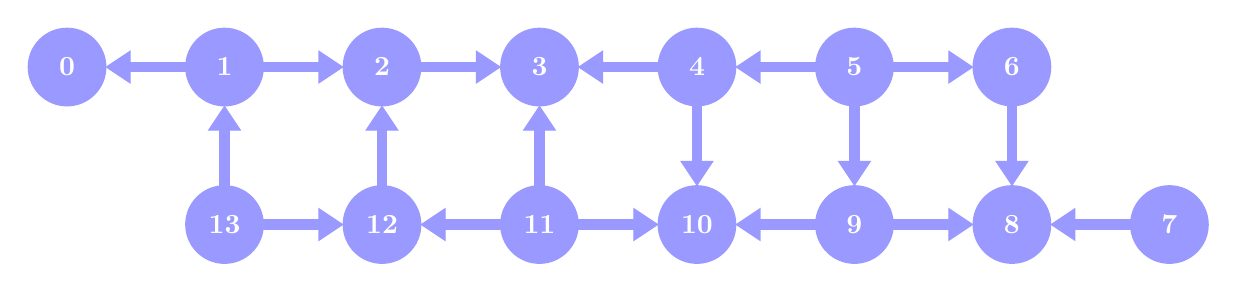
\begin{tikzpicture} %[scale=0.7, transform shape]

\draw[line width=1.3mm, color=blue!40!white] (0.8,0) -- (2,0); \filldraw[color=blue!40!white] (0.5,0) -- (0.8,0.2) -- (0.8,-0.2) -- (0.5,0); %freccia
\draw[line width=1.3mm, color=blue!40!white]  (2,0) -- (4-0.8,0); \filldraw[color=blue!40!white] (3.5,0) -- (3.2,0.2) -- (3.2,-0.2) -- (3.5,0); %freccia
\draw[line width=1.3mm, color=blue!40!white] (4,0) -- (6-0.8,0); \filldraw[color=blue!40!white] (5.5,0) -- (5.2,0.2) -- (5.2,-0.2) -- (5.5,0); %freccia
\draw[line width=1.3mm, color=blue!40!white]  (6+0.8,0) -- (8,0); \filldraw[color=blue!40!white] (6.5,0) -- (6.8,0.2) -- (6.8,-0.2) -- (6.5,0); %freccia
\draw[line width=1.3mm, color=blue!40!white]  (8+0.8,0) -- (10,0); \filldraw[color=blue!40!white] (8.5,0) -- (8.8,0.2) -- (8.8,-0.2) -- (8.5,0); %freccia
\draw[line width=1.3mm, color=blue!40!white]  (10,0) -- (12-0.8,0);  \filldraw[color=blue!40!white] (11.5,0) -- (11.2,0.2) -- (11.2,-0.2) -- (11.5,0); %freccia

\draw[line width=1.3mm, color=blue!40!white]  (2,0-0.8) -- (2,-2);  \filldraw[color=blue!40!white] (2,-0.5) -- (2.2,-0.8) -- (1.8,-0.8) -- (2,-0.5); %freccia
\draw[line width=1.3mm, color=blue!40!white]  (4,0-0.8) -- (4,-2); \filldraw[color=blue!40!white] (4,-0.5) -- (4.2,-0.8) -- (3.8,-0.8) -- (4,-0.5); %freccia
\draw[line width=1.3mm, color=blue!40!white]  (6,0-0.8) -- (6,-2); \filldraw[color=blue!40!white] (6,-0.5) -- (6.2,-0.8) -- (5.8,-0.8) -- (6,-0.5); %freccia
\draw[line width=1.3mm, color=blue!40!white]  (8,0) -- (8,-2+0.8); \filldraw[color=blue!40!white] (8,-1.5) -- (8.2,-1.2) -- (7.8,-1.2) -- (8,-1.5); %freccia
\draw[line width=1.3mm, color=blue!40!white]  (10,0) -- (10,-2+0.8); \filldraw[color=blue!40!white] (10,-1.5) -- (10.2,-1.2) -- (9.8,-1.2) -- (10,-1.5); %freccia
\draw[line width=1.3mm, color=blue!40!white]  (12,0) -- (12,-2+0.8); \filldraw[color=blue!40!white] (12,-1.5) -- (12.2,-1.2) -- (11.8,-1.2) -- (12,-1.5); %freccia


\draw[line width=1.3mm, color=blue!40!white]  (2,-2) -- (4-0.8,-2); \filldraw[color=blue!40!white] (3.5,-2) -- (3.2,0.2-2) -- (3.2,-0.2-2) -- (3.5,-2); %freccia
\draw[line width=1.3mm, color=blue!40!white]  (4+0.8,-2) -- (6,-2); \filldraw[color=blue!40!white] (4.5,-2) -- (4.8,0.2-2) -- (4.8,-0.2-2) -- (4.5,-2); %freccia
\draw[line width=1.3mm, color=blue!40!white]  (6,-2) -- (8-0.8,-2); \filldraw[color=blue!40!white] (7.5,-2) -- (7.2,0.2-2) -- (7.2,-0.2-2) -- (7.5,-2); %freccia
\draw[line width=1.3mm, color=blue!40!white]  (8+0.8,-2) -- (10,-2); \filldraw[color=blue!40!white] (8.5,-2) -- (8.8,0.2-2) -- (8.8,-0.2-2) -- (8.5,-2); %freccia
\draw[line width=1.3mm, color=blue!40!white]  (10,-2) -- (12-0.8,-2); \filldraw[color=blue!40!white] (11.5,-2) -- (11.2,0.2-2) -- (11.2,-0.2-2) -- (11.5,-2); %freccia
\draw[line width=1.3mm, color=blue!40!white]  (12+0.8,-2) -- (14,-2);  \filldraw[color=blue!40!white] (12.5,-2) -- (12.8,0.2-2) -- (12.8,-0.2-2) -- (12.5,-2); %freccia

\fill[fill=blue!40!white] (0,0) circle (0.5cm);
\fill[fill=blue!40!white] (2,0) circle (0.5cm);
\fill[fill=blue!40!white] (4,0) circle (0.5cm);
\fill[fill=blue!40!white] (6,0) circle (0.5cm);
\fill[fill=blue!40!white] (8,0) circle (0.5cm);
\fill[fill=blue!40!white] (10,0) circle (0.5cm);
\fill[fill=blue!40!white] (12,0) circle (0.5cm);


\fill[fill=blue!40!white] (2,-2) circle (0.5cm);
\fill[fill=blue!40!white] (4,-2) circle (0.5cm);
\fill[fill=blue!40!white] (6,-2) circle (0.5cm);
\fill[fill=blue!40!white] (8,-2) circle (0.5cm);
\fill[fill=blue!40!white] (10,-2) circle (0.5cm);
\fill[fill=blue!40!white] (12,-2) circle (0.5cm);
\fill[fill=blue!40!white] (14,-2) circle (0.5cm);


\node[text=white] at (0,0) {\textbf{0}};
\node[text=white] at (2,0) {\textbf{1}};
\node[text=white] at (4,0) {\textbf{2}};
\node[text=white] at (6,0) {\textbf{3}};
\node[text=white] at (8,0) {\textbf{4}};
\node[text=white] at (10,0) {\textbf{5}};
\node[text=white] at (12,0) {\textbf{6}};


\node[text=white] at (2,-2) {\textbf{13}};
\node[text=white] at (4,-2) {\textbf{12}};
\node[text=white] at (6,-2) {\textbf{11}};
\node[text=white] at (8,-2) {\textbf{10}};
\node[text=white] at (10,-2) {\textbf{9}};
\node[text=white] at (12,-2) {\textbf{8}};
\node[text=white] at (14,-2) {\textbf{7}};



\end{tikzpicture}




\end{document}